% Generated by scripts/build_latex.py from report/content.json.
% Statistical values come from results/ and the executed analysis notebook.
\documentclass[11pt,a4paper]{article}
\usepackage[T1]{fontenc}
\usepackage[utf8]{inputenc}
\usepackage{mathptmx,amsmath,amssymb}
\usepackage[left=2cm,right=2cm,top=1.6cm,bottom=1.65cm]{geometry}
\usepackage{graphicx,booktabs,tabularx,array}
\usepackage[table]{xcolor}
\usepackage[colorlinks=true,urlcolor=blue,linkcolor=black]{hyperref}
\graphicspath{{images/}}
\setlength{\parindent}{0pt}
\setlength{\parskip}{5.5pt}
\setlength{\tabcolsep}{4pt}
\renewcommand{\arraystretch}{1.12}
\urlstyle{same}
\hypersetup{pdftitle={Forecasting Kazakhstan's Total Monthly Electricity Generation Using SARIMA},pdfauthor={Mathematics project group, Nazarbayev University}}
\begin{document}
\fontsize{10.5}{13.5}\selectfont

\begin{center}{\bfseries\fontsize{18}{21}\selectfont FORECASTING KAZAKHSTAN'S TOTAL MONTHLY\\ELECTRICITY GENERATION USING SARIMA}\end{center}

\begin{center}{\fontsize{10}{13}\selectfont Mathematics project group\\Nazarbayev University\\Time Series Final Project - 22 November 2026}\end{center}

\textbf{Abstract.} This study compares a seasonal naive baseline with SARIMA for forecasting Kazakhstan's national monthly electricity generation. A frozen Ember dataset contains 102 months, while the main experiment uses 84 observations from 2019 to 2025 after a source audit. Eight low-order specifications are compared using 2024 validation forecasts. SARIMA(1,0,0)(0,1,1)\textsubscript{12} with a constant achieves a 2025 test MAE of 0.343 TWh, compared with 0.435 TWh for the baseline, a 21.1\% reduction. Residual tests reveal no significant autocorrelation at the examined lags. However, prediction intervals under-cover this small test sample, and source construction limits interpretation.\par

\par\vspace{5pt}{\bfseries\fontsize{12.5}{16}\selectfont 1. Introduction}\par\vspace{2pt}

National electricity generation provides a clear application for seasonal time-series forecasting. Short-term forecasts can inform discussion of expected production, although they do not by themselves determine dispatch, consumption or infrastructure requirements. This project asks: \textit{Does SARIMA improve three-month forecasts of Kazakhstan's monthly electricity generation relative to using the same months from the previous year?}\par

The scope is deliberately univariate. The study compares a transparent seasonal benchmark with a small classical model, using the same forecast origins and horizons. The study evaluates whether short-term dependence and a seasonal difference add useful predictive information beyond repeating last year. A source check and a sensitivity analysis support interpretation of the resulting comparison.\par

\par\vspace{5pt}{\bfseries\fontsize{12.5}{16}\selectfont 2. Data description and quality}\par\vspace{2pt}

Ember's public monthly electricity file [1] is filtered to \textit{Area = Kazakhstan} and \textit{Electricity source = Total generation}. The target is \textit{Generation (TWh)}, measured in terawatt-hours. One TWh equals one billion kWh. Dates identify months. The dataset covers the national total, not only Samruk-Energy's own plants.\par

{\fontsize{9.2}{11.3}\selectfont\begin{tabularx}{\linewidth}{@{}>{\hsize=0.64000\hsize\linewidth=\hsize\raggedright\arraybackslash}X>{\hsize=1.36000\hsize\linewidth=\hsize\raggedright\arraybackslash}X@{}}\toprule

\rowcolor[gray]{0.94}

Snapshot audit & Verified result \\

\midrule

Coverage & January 2018-June 2026; 102 months \\

Missingness & No missing months, blank targets or duplicate dates \\

Main experiment & January 2019-December 2025; 84 months \\

Snapshot downloaded & 18 November 2026; preserved as a local CSV \\

\bottomrule\end{tabularx}}\par

{\fontsize{9}{11.3}\selectfont Table 1. Audit of the unchanged national series. The current study uses a frozen data version.\par}

\clearpage

\par\vspace{5pt}{\bfseries\fontsize{12.5}{16}\selectfont 2.1. Source discrepancy and sample choice}\par\vspace{2pt}

The absence of blank cells does not establish measurement quality. Ember lists 9.780 TWh for each of January-March 2018. Samruk's original January report [3] gives 10,357.3 million kWh, or 10.3573 TWh. Its first-quarter report gives 29.3392 TWh, close to Ember's three-month sum of 29.340 TWh. This is consistent with quarterly averaging, but does not prove how the whole file was constructed. The main experiment excludes 2018, keeps the original values unchanged, and checks sensitivity to adding that year back. The partial 2026 year is outside the main experiment so that validation and testing use complete calendar years.\par

\par\vspace{5pt}{\bfseries\fontsize{12.5}{16}\selectfont 2.2. Time-series patterns}\par\vspace{2pt}

\begin{center}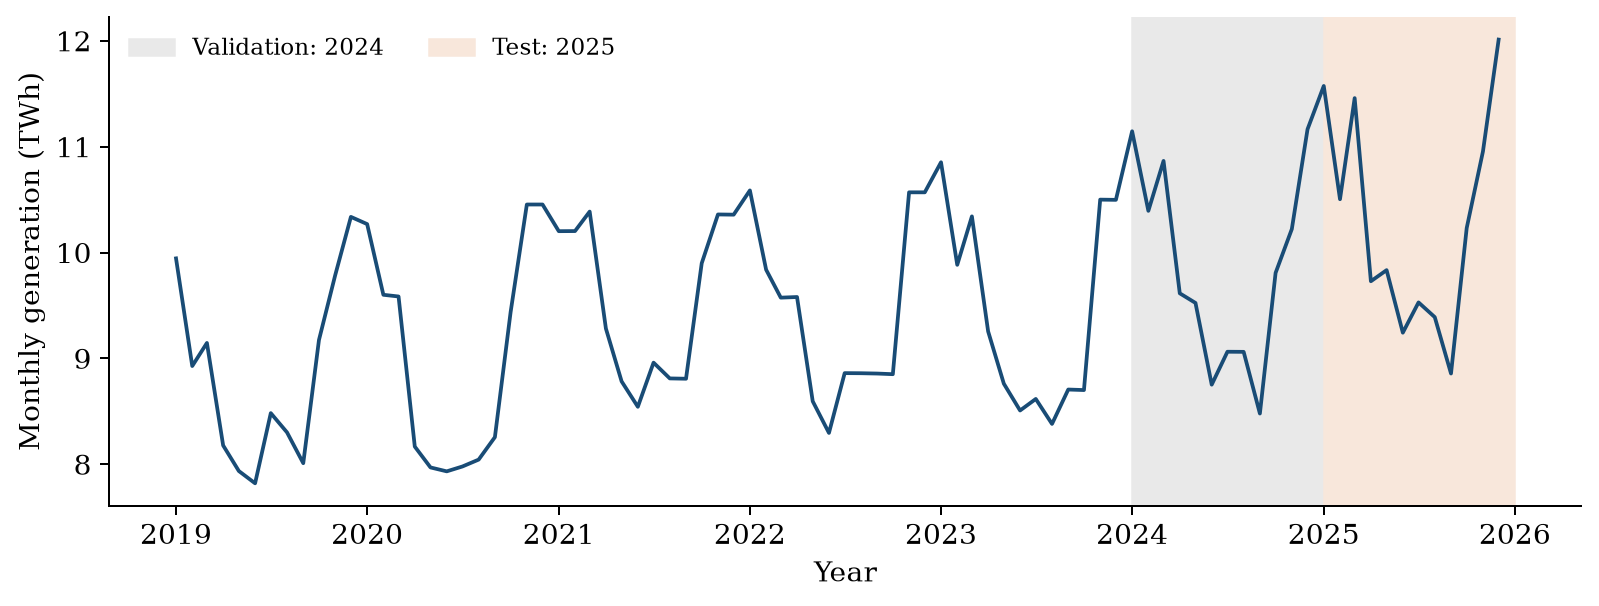
\includegraphics[width=\linewidth,height=5.25cm,keepaspectratio]{01_history.png}\end{center}

{\fontsize{9}{11.3}\selectfont Figure 1. Main study series. Shaded regions mark the validation and test years. The historical display includes all study years, while model exploration uses only 2019-2023.\par}

\begin{center}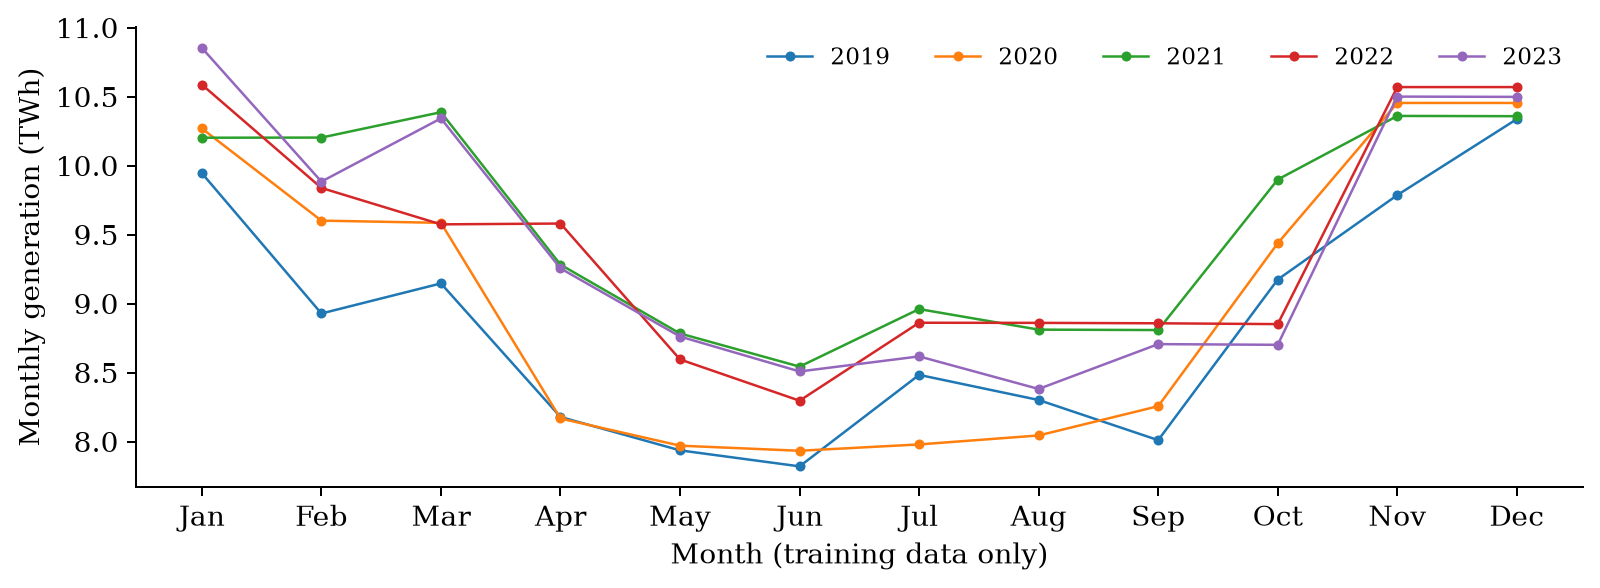
\includegraphics[width=\linewidth,height=5.10cm,keepaspectratio]{02_seasonality.png}\end{center}

{\fontsize{9}{11.3}\selectfont Figure 2. Monthly patterns in the initial training sample. Higher winter values and lower summer values suggest an annual seasonal component. The plot does not establish a causal weather effect.\par}

The training-set lag-12 autocorrelation is 0.681. The ADF test on levels has p = 0.186, while the level-stationarity KPSS test has p >= 0.10. These results alone are inconclusive. After seasonal differencing, the ADF p-value is 0.0008 and the KPSS p-value is 0.095. Together with the plots, this supports considering a seasonal difference. ADF uses a constant, AIC lag selection and maximum lag 8. KPSS uses a constant and automatic bandwidth. Table-limit p-values are bounds.\par

\clearpage

\par\vspace{5pt}{\bfseries\fontsize{12.5}{16}\selectfont 3. Methodology}\par\vspace{2pt}

Let y\textsubscript{t} denote monthly national generation. The seasonal naive forecast repeats last year's matching month. For horizons h = 1, 2, 3 at forecast origin T:\par

\[\widehat{y}_{T+h\mid T}=y_{T+h-12}\tag{1}\]

SARIMA(p,d,q)(P,D,Q)\textsubscript{12} combines ordinary and seasonal autoregressive, differencing and moving-average components [4]. Parameters use state-space maximum likelihood in statsmodels [5], with stationary AR and invertible MA constraints. For the selected model, define z\textsubscript{t} = y\textsubscript{t} - y\textsubscript{t-12}. Then:\par

\[z_t=c+\phi z_{t-1}+\varepsilon_t+\theta\varepsilon_{t-12}\tag{2}\]

The innovations e\textsubscript{t} have mean zero and constant variance under the model. The constant permits an average year-on-year change. No logarithm, external regressor or machine-learning model is used. Eight candidates are fixed before test scoring. The smallest 2024 validation MAE selects the order, with initial-training AICc as a tie-breaker. AICc is not the forecast accuracy measure. Every numerical fit converged.\par

{\fontsize{9.2}{11.3}\selectfont\begin{tabularx}{\linewidth}{@{}>{\hsize=1.02000\hsize\linewidth=\hsize\raggedright\arraybackslash}X>{\hsize=1.41000\hsize\linewidth=\hsize\raggedright\arraybackslash}X>{\hsize=0.57000\hsize\linewidth=\hsize\raggedright\arraybackslash}X@{}}\toprule

\rowcolor[gray]{0.94}

Stage & Dates & Observations \\

\midrule

Initial training & January 2019-December 2023 & 60 \\

Validation / order selection & January-December 2024 & 12 \\

Held-out test & January-December 2025 & 12 \\

\bottomrule\end{tabularx}}\par

{\fontsize{9}{11.3}\selectfont Table 2. Chronological design. Each validation and test year contains four non-overlapping three-month blocks.\par}

Before January, April, July and October, each approach uses observations only through the preceding month. Parameters are refitted on the expanding history, but the selected SARIMA order stays fixed during testing. No actual values from within a three-month block enter that block's forecasts. Earlier observed blocks may enter subsequent fits. Thus horizons 1, 2 and 3 are identical across models. MAE = mean(|y - y-hat|), and RMSE = sqrt(mean((y - y-hat)\textsuperscript{2})); both are in TWh.\par

{\fontsize{9.2}{11.3}\selectfont\begin{tabularx}{\linewidth}{@{}>{\hsize=1.64000\hsize\linewidth=\hsize\raggedright\arraybackslash}X>{\hsize=0.60000\hsize\linewidth=\hsize\raggedright\arraybackslash}X>{\hsize=0.88000\hsize\linewidth=\hsize\raggedright\arraybackslash}X>{\hsize=0.88000\hsize\linewidth=\hsize\raggedright\arraybackslash}X@{}}\toprule

\rowcolor[gray]{0.94}

SARIMA specification & Constant & Validation MAE & Initial AICc \\

\midrule

(1,0,0)(0,1,1) & Yes & 0.354 & 50.70 \\

(0,0,1)(0,1,1) & Yes & 0.358 & 53.74 \\

(1,0,1)(0,1,1) & Yes & 0.378 & 50.08 \\

(1,0,0)(1,1,0) & Yes & 0.400 & 52.78 \\

(1,1,0)(0,1,1) & No & 0.411 & 53.42 \\

(0,1,1)(0,1,1) & No & 0.429 & 48.13 \\

(1,1,0)(1,1,0) & No & 0.456 & 56.82 \\

(0,1,1)(1,1,0) & No & 0.465 & 50.61 \\

\bottomrule\end{tabularx}}\par

{\fontsize{9}{11.3}\selectfont Table 3. Candidate comparison, seasonal period 12 throughout. Seasonal naive validation MAE is 0.508 TWh. AICc values across different differencing orders are descriptive only, not used for cross-order selection.\par}

\clearpage

\par\vspace{5pt}{\bfseries\fontsize{12.5}{16}\selectfont 4. Out-of-sample results}\par\vspace{2pt}

The selected SARIMA(1,0,0)(0,1,1)\textsubscript{12} with a constant yields validation MAE 0.354 TWh. Its specification is then frozen for testing. Across 12 held-out observations in 2025, MAE falls from 0.435 to 0.343 TWh, a reduction of 21.1\%. RMSE falls from 0.483 to 0.418 TWh. These are descriptive improvements for one test year, not a formal finding of universal or statistically significant superiority.\par

{\fontsize{9.2}{11.3}\selectfont\begin{tabularx}{\linewidth}{@{}>{\hsize=1.28000\hsize\linewidth=\hsize\raggedright\arraybackslash}X>{\hsize=0.88000\hsize\linewidth=\hsize\raggedright\arraybackslash}X>{\hsize=0.88000\hsize\linewidth=\hsize\raggedright\arraybackslash}X>{\hsize=0.96000\hsize\linewidth=\hsize\raggedright\arraybackslash}X@{}}\toprule

\rowcolor[gray]{0.94}

Model & MAE (TWh) & RMSE (TWh) & Mean error (TWh) \\

\midrule

Seasonal naive & 0.435 & 0.483 & 0.435 \\

Selected SARIMA & 0.343 & 0.418 & 0.270 \\

\bottomrule\end{tabularx}}\par

{\fontsize{9}{11.3}\selectfont Table 4. Test scores for the same four three-month forecast blocks. Mean error is actual minus forecast, so positive values indicate underprediction.\par}

\begin{center}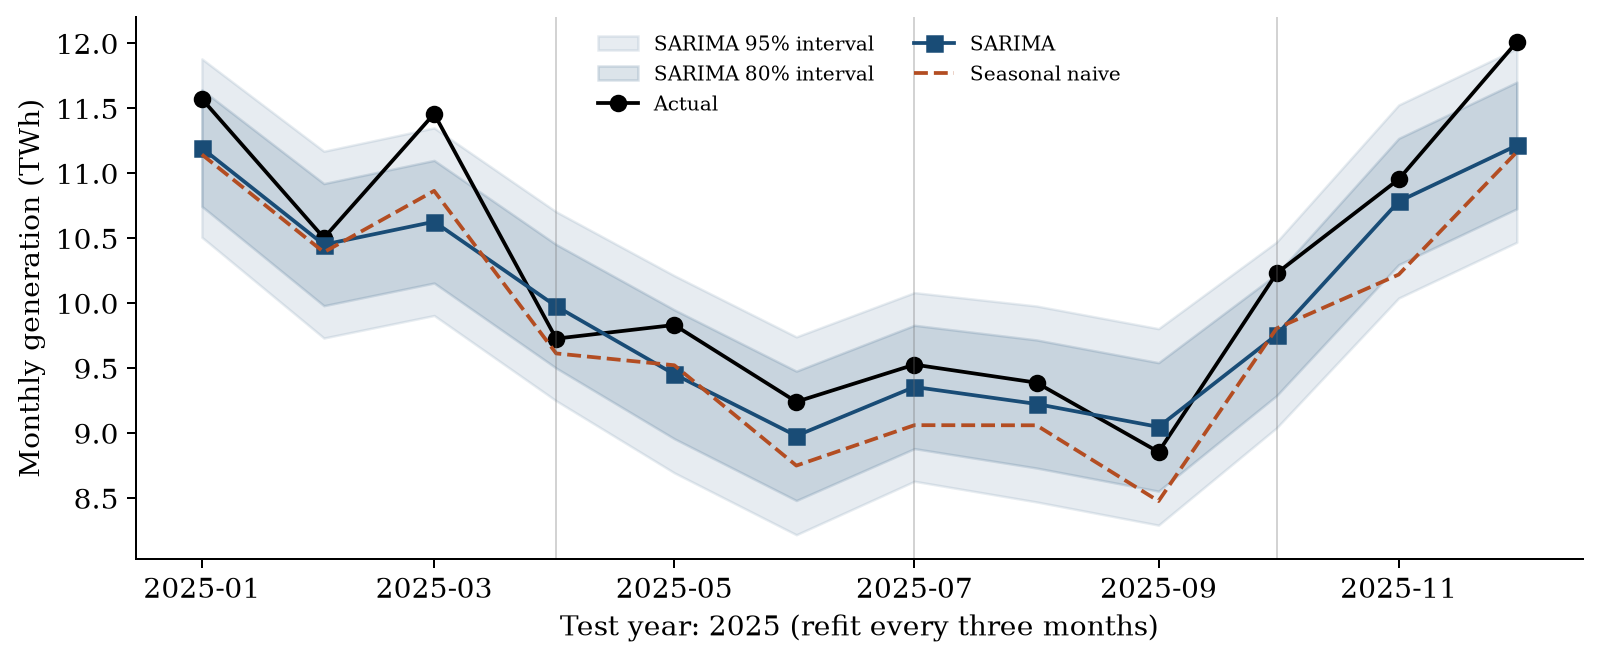
\includegraphics[width=\linewidth,height=7.00cm,keepaspectratio]{04_test_forecasts.png}\end{center}

{\fontsize{9}{11.3}\selectfont Figure 3. Actual and predicted generation in 2025. Shading shows nominal Gaussian SARIMA prediction intervals. Vertical lines separate blocks with newly fitted parameters. Lines connect forecasts from different origins for readability.\par}

{\fontsize{9.2}{11.3}\selectfont\begin{tabularx}{\linewidth}{@{}>{\hsize=1.00000\hsize\linewidth=\hsize\raggedright\arraybackslash}X>{\hsize=1.00000\hsize\linewidth=\hsize\raggedright\arraybackslash}X>{\hsize=1.00000\hsize\linewidth=\hsize\raggedright\arraybackslash}X>{\hsize=1.00000\hsize\linewidth=\hsize\raggedright\arraybackslash}X@{}}\toprule

\rowcolor[gray]{0.94}

Horizon & Observations & Baseline MAE & SARIMA MAE \\

\midrule

1 month(s) & 4 & 0.358 & 0.318 \\

2 month(s) & 4 & 0.370 & 0.191 \\

3 month(s) & 4 & 0.577 & 0.520 \\

\bottomrule\end{tabularx}}\par

{\fontsize{9}{11.3}\selectfont Table 5. Error by horizon, in TWh. With only four observations per horizon, differences are sensitive to individual months.\par}

Both models underpredict on average. Every 2025 monthly total exceeds its 2024 counterpart, which puts the seasonal naive rule at a disadvantage. SARIMA partially adapts to increasing levels, but does not eliminate the bias. The third-month errors remain relatively large. This pattern supports cautious use of a short horizon.\par

\clearpage

\par\vspace{5pt}{\bfseries\fontsize{12.5}{16}\selectfont 5. Model estimates and diagnostics}\par\vspace{2pt}

For a diagnostic view uncontaminated by test observations, the selected specification is fitted through December 2024. Table 6 reports maximum-likelihood estimates and their asymptotic standard errors. These estimates are not the coefficients from every quarterly refit. The seasonal MA estimate is relatively uncertain, which is consistent with the limited number of annual cycles.\par

{\fontsize{9.2}{11.3}\selectfont\begin{tabularx}{\linewidth}{@{}>{\hsize=1.56000\hsize\linewidth=\hsize\raggedright\arraybackslash}X>{\hsize=0.72000\hsize\linewidth=\hsize\raggedright\arraybackslash}X>{\hsize=0.72000\hsize\linewidth=\hsize\raggedright\arraybackslash}X@{}}\toprule

\rowcolor[gray]{0.94}

Parameter & Estimate & Standard error \\

\midrule

Constant c & 0.1214 & 0.0313 \\

AR coefficient phi & 0.3138 & 0.1409 \\

Seasonal MA theta & -0.8640 & 0.3788 \\

Innovation variance (TWh squared) & 0.1162 & 0.0328 \\

\bottomrule\end{tabularx}}\par

{\fontsize{9}{11.3}\selectfont Table 6. Pre-test fit using January 2019-December 2024. In equation (2), c is the intercept of z, not its unconditional mean.\par}

\begin{center}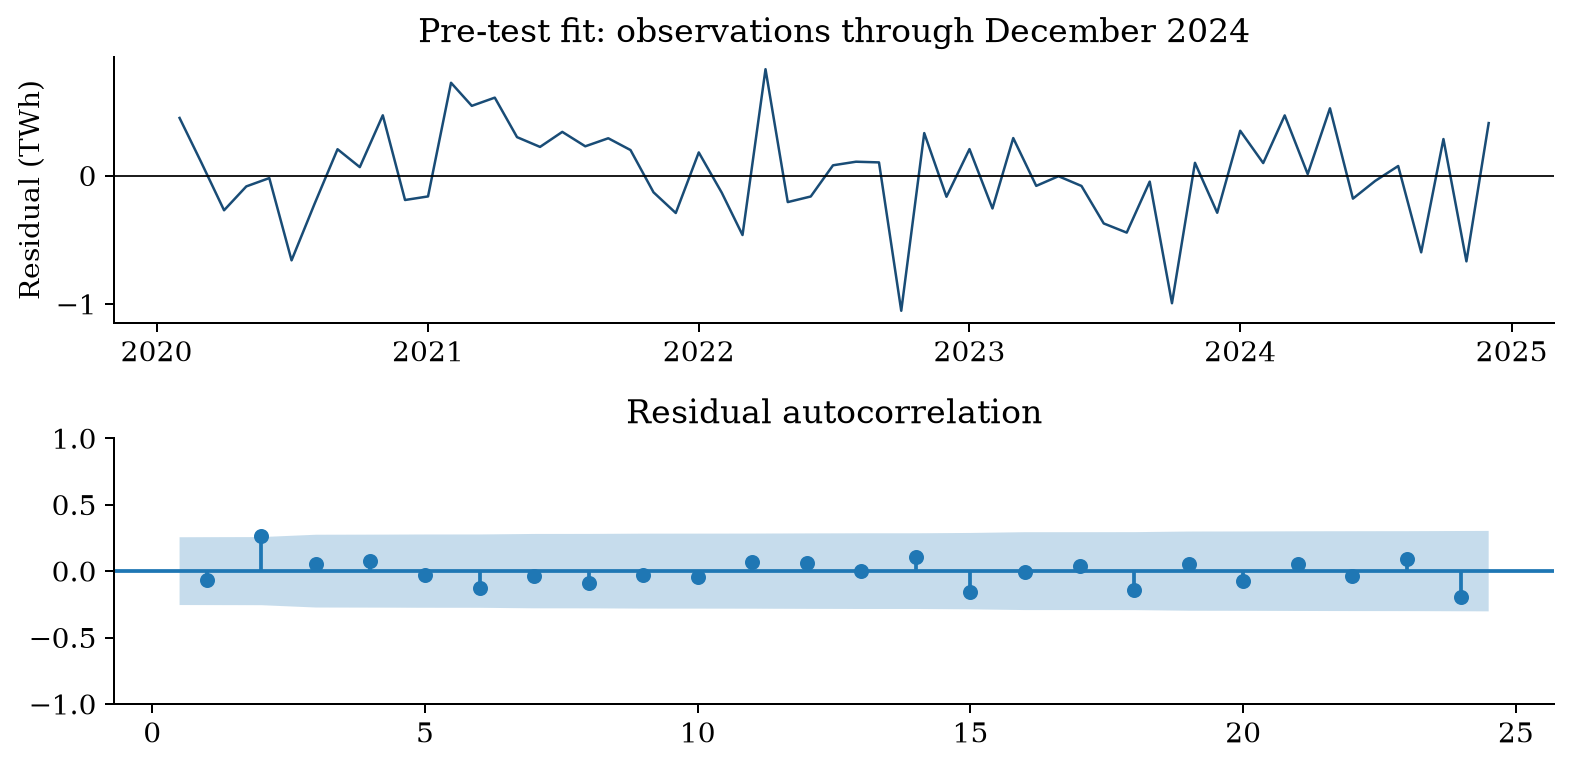
\includegraphics[width=\linewidth,height=7.70cm,keepaspectratio]{05_residuals.png}\end{center}

{\fontsize{9}{11.3}\selectfont Figure 4. Residual sequence and autocorrelation from the pre-test fit. The first 13 residuals are omitted to reduce initialization effects. Remaining residual mean = 0.016 TWh. ACF bounds are approximate individual-lag reference bounds.\par}

Ljung-Box statistics are 8.075 at lag 12 (p = 0.621) and 18.888 at lag 24 (p = 0.652), adjusting degrees of freedom for two AR/MA coefficients. The tests do not reject the absence of residual autocorrelation at these lags. This does not prove independence, normality, constant variance or correct specification. The residual plot and seasonal-source limitations remain relevant.\par

The SARIMA 80\% intervals contain 9 of 12 test observations (75.0\%), and its 95\% intervals contain 10 of 12 (83.3\%). These are nominal Gaussian intervals conditional on the fitted model and estimated parameters. They do not fully reflect parameter uncertainty or data revisions. Coverage below the nominal levels is an important limitation, even though point-forecast errors improve. Twelve observations cannot precisely assess long-run coverage.\par

\clearpage

\par\vspace{5pt}{\bfseries\fontsize{12.5}{16}\selectfont 6. Sensitivity, limitations and conclusion}\par\vspace{2pt}

Adding 2018 back while retaining the selected SARIMA order gives test MAE 0.360 TWh and RMSE 0.441 TWh. The seasonal naive forecasts are unchanged because their matching months lie in 2024. The SARIMA advantage therefore remains, although its magnitude is smaller. This is a sensitivity check, not another model-selection round.\par

The analysis uses a current frozen snapshot, not the data vintages available at each historical forecast origin. Later revisions or source construction may affect past values. Other repeated observations remain after 2018, and only a small part of the source chain was independently checked. Forecasts should therefore be interpreted as forecasts of the published Ember series, not as independently validated measurements of physical generation.\par

A single held-out year and four forecast origins limit generalization. The univariate model does not explain weather, plant outages, fuel supply, trade or policy changes. Monthly totals also reflect unequal month lengths. Generation is not the same as demand, and successful historical forecasts do not establish a causal relationship or an operational planning rule.\par

For illustration, a refit through December 2025 produces the following three-month forecasts. These use only the study endpoint and are deliberately dated. They are not live forecasts made from November 2026 and are not part of the model-selection or main test scores.\par

{\fontsize{9.2}{11.3}\selectfont\begin{tabularx}{\linewidth}{@{}>{\hsize=1.00000\hsize\linewidth=\hsize\raggedright\arraybackslash}X>{\hsize=1.00000\hsize\linewidth=\hsize\raggedright\arraybackslash}X>{\hsize=1.00000\hsize\linewidth=\hsize\raggedright\arraybackslash}X>{\hsize=1.00000\hsize\linewidth=\hsize\raggedright\arraybackslash}X@{}}\toprule

\rowcolor[gray]{0.94}

Forecast month & Forecast (TWh) & 95\% lower & 95\% upper \\

\midrule

2026-01 & 11.860 & 11.130 & 12.590 \\

2026-02 & 10.812 & 10.052 & 11.572 \\

2026-03 & 11.367 & 10.605 & 12.129 \\

\bottomrule\end{tabularx}}\par

{\fontsize{9}{11.3}\selectfont Table 7. Dated forecast illustration, conditional on observations through December 2025.\par}

\textbf{Conclusion.} For this historical evaluation, SARIMA improves three-month point forecasts over the seasonal naive rule, reducing test MAE by 21.1\%. The benefit persists when 2018 is included. Residual autocorrelation tests do not reveal a clear remaining pattern, but the interval coverage and source audit prevent a stronger reliability claim. A longer evaluation across more forecast origins and better-verified monthly source data would be the most useful next steps.\par

\par\vspace{5pt}{\bfseries\fontsize{12.5}{16}\selectfont References}\par\vspace{2pt}

{\fontsize{9}{11.3}\selectfont [1] Ember. Monthly Electricity Data. Snapshot downloaded 18 November 2026. \newline\url{https://ember-energy.org/data/monthly-electricity-data/}\par}

{\fontsize{9}{11.3}\selectfont [2] Ember. Electricity Data Methodology, version 1.6. Kazakhstan source notes. \newline\url{https://files.ember-energy.org/public-downloads/ember_electricity_data_methodology.pdf}\par}

{\fontsize{9}{11.3}\selectfont [3] Samruk-Energy. Electricity market reports, January and January-March 2018. \newline\url{https://samruk-energy.kz/en/press-center/analytical-review}\par}

{\fontsize{9}{11.3}\selectfont [4] Hyndman, R. J. and Athanasopoulos, G. (2021). Forecasting: Principles and Practice, 3rd ed. OTexts. Chapters 5 and 9. \newline\url{https://otexts.com/fpp3/}\par}

{\fontsize{9}{11.3}\selectfont [5] statsmodels. SARIMAX documentation, version 0.15.0. \newline\url{https://www.statsmodels.org/stable/generated/statsmodels.tsa.statespace.sarimax.SARIMAX.html}\par}

\end{document}
